\documentclass[aspectratio=169,11pt]{beamer}

% ═══════════════════════════════════════════════════════════════════════════ %
%  PACKAGES                                                                  %
% ═══════════════════════════════════════════════════════════════════════════ %
\usepackage{amsmath,amssymb,amsfonts}
\usepackage{booktabs}
\usepackage{graphicx}
\usepackage{tikz}
\usetikzlibrary{arrows.meta,positioning,shapes.geometric,calc,fit,
                 decorations.pathreplacing,matrix}
\usepackage{listings}
\usepackage{xcolor}
\usepackage{hyperref}
\usepackage{algorithmic}
\usepackage{multicol}
\usepackage{pgfplots}
\usepackage[normalem]{ulem} % FIXED: Added for \sout (strikethrough) command
\pgfplotsset{compat=1.18}

% ═══════════════════════════════════════════════════════════════════════════ %
%  THEME & COLORS                                                            %
% ═══════════════════════════════════════════════════════════════════════════ %
\usetheme{Madrid}
\usecolortheme{whale}

\definecolor{deepgreen}{RGB}{0,120,60}
\definecolor{deepred}{RGB}{180,30,30}
\definecolor{deepblue}{RGB}{30,60,150}
\definecolor{codebg}{RGB}{245,245,250}
\definecolor{accent}{RGB}{220,80,40}
\definecolor{gold}{RGB}{180,140,20}
\definecolor{lightgray}{RGB}{240,240,240}

\setbeamercolor{block title}{bg=deepblue,fg=white}
\setbeamercolor{block body}{bg=lightgray}
\setbeamercolor{block title alerted}{bg=deepred,fg=white}
\setbeamercolor{block body alerted}{bg=lightgray}
\setbeamercolor{block title example}{bg=deepgreen,fg=white}
\setbeamercolor{block body example}{bg=lightgray}

\lstset{
    language=Python,
    basicstyle=\ttfamily\tiny,
    keywordstyle=\color{deepblue}\bfseries,
    commentstyle=\color{deepgreen}\itshape,
    stringstyle=\color{accent},
    backgroundcolor=\color{codebg},
    frame=single,
    breaklines=true,
    showstringspaces=false,
    numbers=left,
    numberstyle=\tiny\color{gray},
    tabsize=4,
}

% ═══════════════════════════════════════════════════════════════════════════ %
%  TITLE                                                                     %
% ═══════════════════════════════════════════════════════════════════════════ %
\title[MoE Kernel Optimization]{\textbf{Optimizing Mixture-of-Experts Kernels}\\
\large From First Principles to B200 Tensor Cores}
\subtitle{FlashInfer MoE Challenge --- DeepSeek-V3/R1 Architecture}
\author[V. Nawander]{Presentation by Vansh Nawander}
\date{April 2026}
\institute[Humming Bird Team]{Humming Bird Team \\ GPU Kernel Engineering}

\begin{document}

% ═══════════════════════════════════════════════════════════════════════════ %
%  TITLE SLIDE                                                               %
% ═══════════════════════════════════════════════════════════════════════════ %
\begin{frame}
\titlepage
\end{frame}

% ═══════════════════════════════════════════════════════════════════════════ %
%  OUTLINE                                                                   %
% ═══════════════════════════════════════════════════════════════════════════ %
\begin{frame}{Outline}
\tableofcontents
\end{frame}

\begin{frame}{Team Details}
\begin{block}{Project Team}
\begin{itemize}
    \item \textbf{Team Name:} Humming Bird Team
    \item \textbf{Presenter:} Vansh Nawander
    \item \textbf{Focus:} End-to-end optimization of DeepSeek MoE kernels on B200
\end{itemize}
\end{block}

\begin{columns}[T]
\column{0.48\textwidth}
\begin{exampleblock}{What This Talk Covers}
\begin{itemize}
    \item Mathematical specification and precision chain
    \item Optimization journey from Sub-7 to Sub-12
    \item Failures, fixes, and validated trade-offs
\end{itemize}
\end{exampleblock}

\column{0.48\textwidth}
\begin{alertblock}{Success Criteria}
\begin{itemize}
    \item Numerical correctness under challenge tolerance
    \item Better throughput and lower memory traffic
    \item Stable execution without runtime/compiler regressions
\end{itemize}
\end{alertblock}
\end{columns}
\end{frame}

% ═══════════════════════════════════════════════════════════════════════════ %
\section{Problem Statement \& Challenge Context}
% ═══════════════════════════════════════════════════════════════════════════ %

\begin{frame}[t]{The FlashInfer MoE Challenge (Setup)}
\small
\begin{block}{Objective}
Write the fastest correct Triton kernel for a \textbf{Mixture-of-Experts (MoE)
feed-forward layer} from DeepSeek-V3/R1 on NVIDIA B200 GPUs.
\end{block}

\begin{columns}[T]
\column{0.48\textwidth}
\textbf{Architecture Parameters}
\begin{itemize}
    \item Hidden size $H = 7168$
    \item Intermediate size $I = 2048$
    \item Total experts $E = 256$
    \item Local experts $E_L = 32$
    \item Top-K $= 8$ experts per token
    \item $N_{\text{group}} = 8$, Top-K groups $= 4$
    \item Block quantization $Q = 128$
\end{itemize}

\column{0.48\textwidth}
\textbf{Data Types}
\begin{itemize}
    \item Hidden states: \texttt{FP8 E4M3} + FP32 scales
    \item Expert weights: \texttt{FP8 E4M3} + FP32 scales
    \item Routing: \texttt{BF16} logits + bias
    \item Output: \texttt{BF16}
    \item Intermediate compute: \texttt{FP32}
\end{itemize}
\end{columns}
\end{frame}

\begin{frame}[t]{The FlashInfer MoE Challenge (Hardware Targets)}
\small
\begin{block}{Target Hardware: NVIDIA B200}
\begin{itemize}
    \item 148 SMs
    \item Up to 4.5 PFLOPS FP8 tensor-core throughput
    \item About 228 KB shared memory per SM
    \item About 8 TB/s HBM bandwidth
\end{itemize}
\end{block}

\begin{exampleblock}{Optimization Focus}
Balance three objectives simultaneously: numerical correctness, memory efficiency,
and launch/occupancy efficiency.
\end{exampleblock}
\end{frame}

% ═══════════════════════════════════════════════════════════════════════════ %
\begin{frame}[t]{Why MoE Kernels Are Hard}
\small
\begin{columns}[T]
\column{0.55\textwidth}

\begin{alertblock}{Five Fundamental Challenges}
\begin{enumerate}
    \item \textbf{Load Imbalance:} Expert A gets 500 tokens, Expert B gets 3 
    --- wildly different GEMM sizes
    \item \textbf{Scatter/Gather:} Tokens gathered per-expert, results scattered 
    back --- memory-unfriendly random access
    \item \textbf{FP8 Block-Scale Dequant:} Can't call standard cuBLAS --- need 
    custom per-block scale handling inside GEMM
    \item \textbf{Kernel Launch Overhead:} 32 experts $\times$ 3 ops $=$ 96 
    launches $\times$ 5$\mu$s $=$ 480$\mu$s wasted
    \item \textbf{Tile Waste:} Expert with $T_k=5$ tokens wastes 92\% of a 
    $64\times128$ GEMM tile
\end{enumerate}
\end{alertblock}

\column{0.42\textwidth}
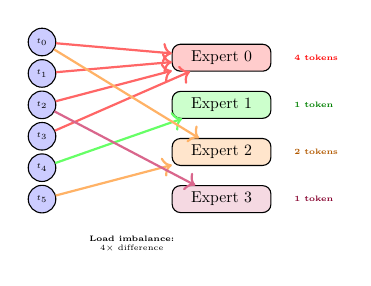
\begin{tikzpicture}[scale=0.57, transform shape,
    expert/.style={rectangle, draw, minimum width=2.2cm, minimum height=0.6cm, 
                   rounded corners=3pt},
    token/.style={circle, draw, fill=blue!20, minimum size=0.35cm, 
                  font=\tiny}]
    
    % Tokens
    \foreach \i in {0,...,5} {
        \node[token] (t\i) at (0, -\i*0.7) {$t_{\i}$};
    }
    
    % Experts
    \node[expert, fill=red!20] (e0) at (4, -0.35) {Expert 0};
    \node[expert, fill=green!20] (e1) at (4, -1.4) {Expert 1};
    \node[expert, fill=orange!20] (e2) at (4, -2.45) {Expert 2};
    \node[expert, fill=purple!15] (e3) at (4, -3.5) {Expert 3};
    
    % Connections (showing imbalance)
    \draw[->, thick, red!60] (t0) -- (e0);
    \draw[->, thick, red!60] (t1) -- (e0);
    \draw[->, thick, red!60] (t2) -- (e0);
    \draw[->, thick, red!60] (t3) -- (e0);
    \draw[->, thick, green!60] (t4) -- (e1);
    \draw[->, thick, orange!60] (t0) -- (e2);
    \draw[->, thick, orange!60] (t5) -- (e2);
    \draw[->, thick, purple!60] (t2) -- (e3);
    
    % Labels
    \node[right, font=\tiny\bfseries, red] at (5.5, -0.35) {4 tokens};
    \node[right, font=\tiny\bfseries, green!50!black] at (5.5, -1.4) {1 token};
    \node[right, font=\tiny\bfseries, orange!70!black] at (5.5, -2.45) {2 tokens};
    \node[right, font=\tiny\bfseries, purple!70!black] at (5.5, -3.5) {1 token};
    
    \node[font=\tiny, align=center] at (2, -4.5) {\textbf{Load imbalance:}\\4$\times$ difference};
\end{tikzpicture}
\end{columns}
\end{frame}

% ═══════════════════════════════════════════════════════════════════════════ %
\section{Mathematical Foundations}
% ═══════════════════════════════════════════════════════════════════════════ %

\begin{frame}[t]{Complete Mathematical Specification (I)}
\small
\begin{block}{Stage 1: FP8 Block-Scale Dequantization}
\vspace{-0.2cm}
\begin{align}
X_{\text{real}}[t, j] &= X_{\text{fp8}}[t, j] \times S_X\!\left[\left\lfloor j/128 \right\rfloor,\; t\right]
\end{align}
\vspace{-0.2cm}
\begin{itemize}
    \item Each block of 128 columns shares one FP32 scale factor
    \item $S_X$ shape: $(56, T)$ where $56 = 7168/128$
    \item Dequantization is performed just-in-time inside compute kernels
\end{itemize}
\end{block}

\begin{exampleblock}{Implementation Note}
The block size is chosen to align with tensor-core-friendly tile geometry, so scale fetches stay lightweight and cache-friendly.
\end{exampleblock}
\end{frame}

\begin{frame}[t]{Complete Mathematical Specification (II)}
\small
\begin{block}{Stage 2: Grouped Top-K Routing}
\vspace{-0.2cm}
\begin{align}
s &= \sigma(R) \in [0,1]^{T \times 256} \\
s_{\text{bias}} &= s + B \\
\text{score}_g &= \sum \text{top-}2(s_{\text{bias}}[\cdot, g \cdot 32:(g{+}1) \cdot 32])
\quad \forall\, g \in \{0,\dots,7\} \\
\text{groups}_{\text{sel}} &= \text{top-}4(\text{score}_g) \\
\text{idx}_{\text{top8}} &= \text{top-}8\!\left(\text{masked}(s_{\text{bias}})\right) \\
w_k &= \frac{s[\text{idx}_k]}{\sum_{j=1}^{8} s[\text{idx}_j]} \times \alpha
\end{align}
\end{block}

\begin{alertblock}{Why Group Filtering Matters}
Selecting top groups before top experts reduces candidate search width and keeps routing cost bounded while preserving quality.
\end{alertblock}
\end{frame}

% ═══════════════════════════════════════════════════════════════════════════ %
\begin{frame}[t]{Expert FFN: The Core Computation (I)}
\small
\begin{block}{Stage 3: Per-Expert Feed-Forward (expert $e$ with $T_k$ tokens)}
\vspace{-0.2cm}
\begin{align}
\textbf{GEMM1:} \quad Y_1 &= X_e \cdot W_{1,e}^\top
\in \mathbb{R}^{T_k \times 4096} \\
\textbf{Split:} \quad \text{gate} &= Y_1[:, :2048], \quad \text{up}=Y_1[:, 2048:] \\
\textbf{SwiGLU:} \quad C &= \text{gate} \odot \text{silu}(\text{up})
= \text{gate} \odot (\text{up}\cdot\sigma(\text{up})) \\
\textbf{GEMM2:} \quad Y_2 &= C \cdot W_{2,e}^\top
\in \mathbb{R}^{T_k \times 7168}
\end{align}
\end{block}

\begin{itemize}
    \item GEMM1 expands to gate+up channels in one pass
    \item SwiGLU is applied before projection back to hidden dimension
\end{itemize}
\end{frame}

\begin{frame}[t]{Expert FFN: The Core Computation (II)}
\small
\begin{block}{Stage 4: Weighted Scatter-Add}
\vspace{-0.2cm}
\begin{equation}
\text{output}[t] = \sum_{e \in \text{top-8}(t)} w_{t,e} \cdot Y_{2,e}[t]
\end{equation}
\end{block}

\begin{exampleblock}{Why $W_1$ is $(4096 \times 7168)$, not $(2048 \times 7168)$}
SwiGLU needs two projections (gate and up). DeepSeek fuses both in one matrix:
rows $[0{:}2048]$ for gate and rows $[2048{:}4096]$ for up.
\end{exampleblock}

\begin{alertblock}{Practical Implication}
Each token may contribute through multiple experts, so the final scatter-add must preserve numerical stability and deterministic accumulation behavior.
\end{alertblock}
\end{frame}

% ═══════════════════════════════════════════════════════════════════════════ %
\begin{frame}{FP8 Block-Scale Dequantization Inside GEMM}
\begin{columns}[T]
\column{0.55\textwidth}
\begin{block}{The Block-Scale Scheme}
Every $128 \times 128$ tile of the weight matrix shares one FP32 scale:
\[
W_{\text{real}}[n, k] = W_{\text{fp8}}[n, k] \times S_W\!\left[\left\lfloor n/128 \right\rfloor, 
\left\lfloor k/128 \right\rfloor\right]
\]
\end{block}

\vspace{0.2cm}

When \texttt{BLOCK\_N} $=$ \texttt{BLOCK\_K} $= 128 = $ \texttt{BLOCK\_Q}:
\begin{itemize}
    \item Each GEMM tile maps to \textbf{exactly one scale value}
    \item Scale load becomes a \textbf{scalar load} (4 bytes!)
    \item This is why tile sizes are carefully chosen
\end{itemize}

\column{0.42\textwidth}
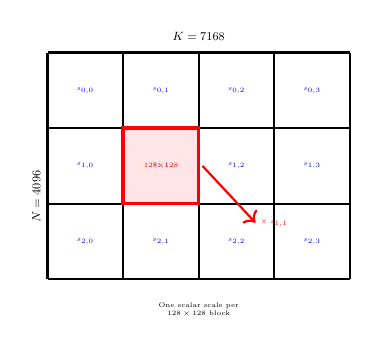
\begin{tikzpicture}[scale=0.48, transform shape]
    % Weight matrix grid
    \draw[step=2, thick] (0,0) grid (8, -6);
    
    % Labels
    \node[above, font=\small\bfseries] at (4, 0.2) {$K = 7168$};
    \node[left, font=\small\bfseries, rotate=90] at (-0.3, -3) {$N = 4096$};
    
    % Scale annotations
    \foreach \i in {0,...,3} {
        \foreach \j in {0,...,2} {
            \node[font=\tiny, blue] at (\i*2+1, -\j*2-1) 
                {$s_{\j,\i}$};
        }
    }
    
    % Highlight one block
    \fill[red!20, opacity=0.5] (2, -2) rectangle (4, -4);
    \draw[red, very thick] (2, -2) rectangle (4, -4);
    \node[font=\tiny\bfseries, red] at (3, -3) {$128{\times}128$};
    
    % Arrow to scale
    \draw[->, thick, red] (4.1, -3) -- (5.5, -4.5) 
        node[right, font=\tiny] {$\times\; s_{1,1}$};
    
    \node[below, font=\tiny, align=center] at (4, -6.5) 
        {One scalar scale per\\$128\times128$ block};
\end{tikzpicture}
\end{columns}
\end{frame}

% ═══════════════════════════════════════════════════════════════════════════ %
\section{Optimization Journey: Submissions 7--12}
% ═══════════════════════════════════════════════════════════════════════════ %

\begin{frame}[t]{Submission Timeline Overview (Chronology)}
\begin{center}
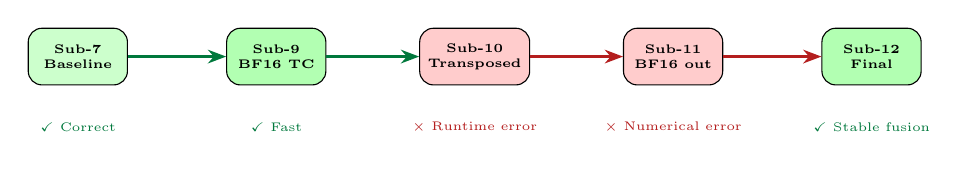
\begin{tikzpicture}[
    sub/.style={rectangle, draw, rounded corners=5pt, minimum width=1.4cm,
                minimum height=0.8cm, font=\tiny\bfseries, align=center},
    arrow/.style={->, thick, >=Stealth},
    label/.style={font=\tiny, align=center},
    scale=0.9, transform shape
]
\node[sub, fill=green!20] (s7) at (0,0) {Sub-7\\Baseline};
\node[sub, fill=green!30] (s9) at (2.8,0) {Sub-9\\BF16 TC};
\node[sub, fill=red!20] (s10) at (5.6,0) {Sub-10\\Transposed};
\node[sub, fill=red!20] (s11a) at (8.4,0) {Sub-11\\BF16 out};
\node[sub, fill=green!30] (s12) at (11.2,0) {Sub-12\\Final};
\draw[arrow, deepgreen] (s7) -- (s9);
\draw[arrow, deepgreen] (s9) -- (s10);
\draw[arrow, deepred] (s10) -- (s11a);
\draw[arrow, deepred] (s11a) -- (s12);
\node[label, deepgreen] at (0, -1) {\checkmark\ Correct};
\node[label, deepgreen] at (2.8, -1) {\checkmark\ Fast};
\node[label, deepred] at (5.6, -1) {$\times$ Runtime error};
\node[label, deepred] at (8.4, -1) {$\times$ Numerical error};
\node[label, deepgreen] at (11.2, -1) {\checkmark\ Stable fusion};
\end{tikzpicture}
\end{center}
\end{frame}

\begin{frame}[t]{Submission Timeline Overview (Outcomes)}
\small
\begin{columns}[T]
\column{0.48\textwidth}
\begin{exampleblock}{What Worked}
\begin{itemize}
    \item FP8 $\to$ BF16 lossless promotion
    \item Post-dot FP32 scale application
    \item Fused GEMM1 + SwiGLU kernel
    \item FP8 bulk gather
    \item Route-weight fusion in GEMM2 epilogue
\end{itemize}
\end{exampleblock}
\column{0.48\textwidth}
\begin{alertblock}{What Failed}
\begin{itemize}
    \item Transposed pointer loads
    \item BF16 SwiGLU output
    \item \texttt{tl.atomic\_add} 2D scatter
    \item Non-constexpr persistent loop path
    \item Over-aggressive \texttt{num\_stages}
\end{itemize}
\end{alertblock}
\end{columns}
\end{frame}

% ═══════════════════════════════════════════════════════════════════════════ %
\begin{frame}[t]{Key Insight \#1: The Factored Scale Trick}
\footnotesize

\begin{block}{The Problem: BF16 Tensor Cores vs.\ FP32 Precision}
\vspace{-0.2cm}
\begin{align*}
\text{result}[m,n] &= \sum_k \underbrace{\left(a_{\text{fp8}}[m,k] \times S_a[m, \lfloor k/128\rfloor]\right)}_{\text{dequant to FP32}} 
    \times \underbrace{\left(w_{\text{fp8}}[n,k] \times S_w[\lfloor n/128\rfloor, \lfloor k/128\rfloor]\right)}_{\text{dequant to FP32}}
\end{align*}
\vspace{-0.2cm}
Na\"ive approach: dequant $\to$ FP32 $\to$ truncate to BF16 $\to$ dot. 
\textcolor{deepred}{\textbf{Loses 16 bits of scale precision!}}
\end{block}

\begin{exampleblock}{The Solution: Factor Out Scales}
\vspace{-0.2cm}
\begin{align*}
\text{result}[m,n] &= \sum_{\text{blk}} 
    \underbrace{S_a[m, \text{blk}] \times S_w[\lfloor n/128\rfloor, \text{blk}]}_{\text{FP32 post-multiply}} 
    \times \sum_{k' \in \text{blk}} 
    \underbrace{a_{\text{fp8}}[m,k'] \times w_{\text{fp8}}[n,k']}_{\text{BF16 dot product}}
\end{align*}
\vspace{-0.2cm}
\begin{itemize}
    \item FP8 $\to$ BF16 is \textbf{lossless} (4 sig.\ bits $\to$ 8-bit container)
    \item BF16 $\times$ BF16 multiply preserves all 4+4 meaningful bits
    \item Scales applied in \textbf{full FP32 after the dot} --- zero precision loss
    \item Result: BF16 tensor core speed with FP32-equivalent precision
\end{itemize}
\end{exampleblock}
\end{frame}

% ═══════════════════════════════════════════════════════════════════════════ %
\begin{frame}[t]{Key Insight \#1: Visual Data Flow (Diagram)}
\begin{center}
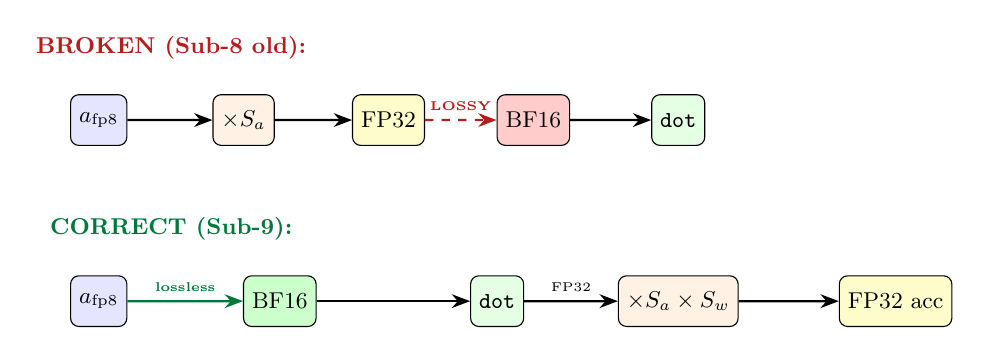
\begin{tikzpicture}[
    box/.style={rectangle, draw, rounded corners=3pt, minimum height=0.7cm,
                font=\small, align=center},
    arrow/.style={->, thick, >=Stealth},
    scale=0.92, transform shape
]
\node[font=\small\bfseries, deepred] at (-5, 2.5) {BROKEN (Sub-8 old):};
\node[box, fill=blue!10] (a1) at (-6, 1.5) {$a_{\text{fp8}}$};
\node[box, fill=orange!10] (s1) at (-4, 1.5) {$\times S_a$};
\node[box, fill=yellow!20] (f1) at (-2, 1.5) {FP32};
\node[box, fill=red!20] (b1) at (0, 1.5) {BF16};
\node[box, fill=green!10] (d1) at (2, 1.5) {\texttt{dot}};
\draw[arrow] (a1) -- (s1);
\draw[arrow] (s1) -- (f1);
\draw[arrow, deepred, dashed] (f1) -- node[above, font=\tiny\bfseries, deepred] {LOSSY} (b1);
\draw[arrow] (b1) -- (d1);

\node[font=\small\bfseries, deepgreen] at (-5, 0.0) {CORRECT (Sub-9):};
\node[box, fill=blue!10] (a2) at (-6, -1) {$a_{\text{fp8}}$};
\node[box, fill=green!20] (b2) at (-3.5, -1) {BF16};
\node[box, fill=green!10] (d2) at (-0.5, -1) {\texttt{dot}};
\node[box, fill=orange!10] (s2) at (2, -1) {$\times S_a \times S_w$};
\node[box, fill=yellow!20] (f2) at (5, -1) {FP32 acc};
\draw[arrow, deepgreen] (a2) -- node[above, font=\tiny\bfseries, deepgreen] {lossless} (b2);
\draw[arrow] (b2) -- (d2);
\draw[arrow] (d2) -- node[above, font=\tiny] {FP32} (s2);
\draw[arrow] (s2) -- (f2);
\end{tikzpicture}
\end{center}
\end{frame}

\begin{frame}[t]{Key Insight \#1: Visual Data Flow (Comparison)}
\begin{center}
\begin{tabular}{lcc}
\toprule
\textbf{Property} & \textbf{Broken Path} & \textbf{Correct Path} \\
\midrule
Scale precision & 7-bit (BF16) & 23-bit (FP32) \\
Input precision & Truncated & Lossless \\
Tensor cores & Under-utilized & Useful/accurate \\
Error over $K{=}7168$ & Compounds & Bounded \\
\bottomrule
\end{tabular}
\end{center}
\end{frame}

% ═══════════════════════════════════════════════════════════════════════════ %
\begin{frame}[t]{Key Insight \#2: Fused GEMM1 + SwiGLU (Diagram)}
\small
\begin{columns}[T]
\column{0.49\textwidth}
\textbf{Before (2 kernels)}
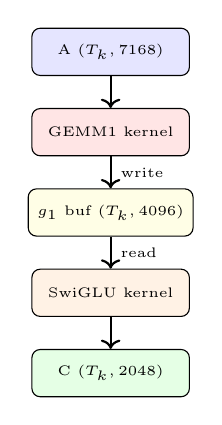
\begin{tikzpicture}[
    box/.style={rectangle, draw, rounded corners=3pt, minimum width=2cm,
                minimum height=0.6cm, font=\tiny, align=center},
    arrow/.style={->, thick},
    scale=0.85
]
\node[box, fill=blue!10] (a) at (0, 0) {A ($T_k, 7168$)};
\node[box, fill=red!10] (g1) at (0, -1.2) {GEMM1 kernel};
\node[box, fill=yellow!10] (buf) at (0, -2.4) {$g_1$ buf ($T_k, 4096$)};
\node[box, fill=orange!10] (sw) at (0, -3.6) {SwiGLU kernel};
\node[box, fill=green!10] (c) at (0, -4.8) {C ($T_k, 2048$)};
\draw[arrow] (a) -- (g1);
\draw[arrow] (g1) -- node[right, font=\tiny] {write} (buf);
\draw[arrow] (buf) -- node[right, font=\tiny] {read} (sw);
\draw[arrow] (sw) -- (c);
\end{tikzpicture}

\column{0.49\textwidth}
\textbf{After (fused)}
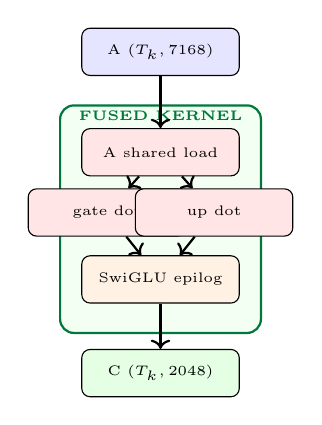
\begin{tikzpicture}[
    box/.style={rectangle, draw, rounded corners=3pt, minimum width=2cm,
                minimum height=0.6cm, font=\tiny, align=center},
    arrow/.style={->, thick},
    scale=0.85
]
\node[box, fill=blue!10] (a) at (0, 0) {A ($T_k, 7168$)};
\draw[rounded corners=5pt, fill=green!5, draw=deepgreen, thick]
    (-1.5, -0.8) rectangle (1.5, -4.2);
\node[font=\tiny\bfseries, deepgreen] at (0, -0.95) {FUSED KERNEL};
\node[box, fill=red!10] (g) at (0, -1.5) {A shared load};
\node[box, fill=red!10] (g1) at (-0.8, -2.4) {gate dot};
\node[box, fill=red!10] (g2) at (0.8, -2.4) {up dot};
\node[box, fill=orange!10] (sw) at (0, -3.4) {SwiGLU epilog};
\node[box, fill=green!10] (c) at (0, -4.8) {C ($T_k, 2048$)};
\draw[arrow] (a) -- (g);
\draw[arrow] (g) -- (g1);
\draw[arrow] (g) -- (g2);
\draw[arrow] (g1) -- (sw);
\draw[arrow] (g2) -- (sw);
\draw[arrow] (sw) -- (c);
\end{tikzpicture}
\end{columns}
\end{frame}

\begin{frame}[t]{Key Insight \#2: Fused GEMM1 + SwiGLU (Impact)}
\small
\begin{block}{Bandwidth Savings (per expert, $T_k = 256$)}
\begin{itemize}
    \item Eliminated $g_1$ buffer write+read: $256 \times 4096 \times 4 \times 2 = 8.4$ MB
    \item Halved A loads per K-iteration (shared for gate and up)
    \item Removed one kernel launch ($\sim$5--10 $\mu$s)
\end{itemize}
\end{block}

\begin{exampleblock}{Net Effect}
Fusion improves both memory efficiency and launch amortization, especially for small and medium $T_k$ where overhead is non-negligible.
\end{exampleblock}
\end{frame}

% ═══════════════════════════════════════════════════════════════════════════ %
\begin{frame}[fragile,t]{Key Insight \#3: Memory Coalescing Matters (Code View)}
\small
\begin{columns}[T]
\column{0.48\textwidth}
\begin{exampleblock}{Coalesced Load (Sub-9)}
\begin{lstlisting}[basicstyle=\ttfamily\scriptsize]
# W stored as (N, K), stride=(K, 1)
w = tl.load(w_ptr
    + offs_n[:, None] * K
    + offs_k[None, :] * 1)
# contiguous accesses in k
\end{lstlisting}
Then: \texttt{tl.dot(a, tl.trans(w))}
\end{exampleblock}

\column{0.48\textwidth}
\begin{alertblock}{Transposed Load (Sub-10)}
\begin{lstlisting}[basicstyle=\ttfamily\scriptsize]
w_t = tl.load(w_ptr
    + offs_k[:, None] * 1
    + offs_n[None, :] * K)
# strided accesses in memory
\end{lstlisting}
Then: \texttt{tl.dot(a, w\_t)}
\end{alertblock}
\end{columns}
\end{frame}

\begin{frame}[t]{Key Insight \#3: Memory Coalescing Matters (Bandwidth Impact)}
\begin{center}
\begin{tabular}{lcc}
\toprule
& \textbf{Coalesced + trans} & \textbf{Transposed load} \\
\midrule
Useful data/tile & 16 KB & 16 KB \\
Actual HBM read & $\sim$64 KB & $\sim$2 MB \\
Amplification & 4$\times$ & 128$\times$ \\
Per expert (56 K-iters) & 7 MB & 224 MB \\
20 experts total & 140 MB & 4.5 GB (timeout-prone) \\
\bottomrule
\end{tabular}
\end{center}
\end{frame}

% ═══════════════════════════════════════════════════════════════════════════ %
\begin{frame}[t,shrink=8]{Key Insight \#4: Shared Memory Budget}
\scriptsize

\begin{block}{SMEM Per Pipeline Stage}
\vspace{-0.2cm}
\[
\text{SMEM}_{\text{stage}} = \underbrace{\text{BLOCK\_M} \times \text{BLOCK\_K} \times \text{sizeof}(A)}_{\text{A tile}} 
+ \underbrace{\text{BLOCK\_N} \times \text{BLOCK\_K} \times \text{sizeof}(W)}_{\text{W tile(s)}}
\]
\[
\text{SMEM}_{\text{total}} = \text{SMEM}_{\text{stage}} \times \texttt{num\_stages} 
    + \text{compiler overhead}
\]
Must be $< 228$ KB (B200 limit per SM).
\end{block}

\vspace{0.2cm}

\begin{center}
\scriptsize
\begin{tabular}{lccccc}
\toprule
\textbf{Kernel} & \textbf{A type} & \textbf{Per stage} & \textbf{Stages} & 
    \textbf{Total} & \textbf{Status} \\
\midrule
GEMM1+SwiGLU (FP8 A) & FP8 & 8+16+16=40 KB & 3 & 120 KB & 
    \textcolor{deepgreen}{\checkmark} \\
GEMM1+SwiGLU (FP32 A) & FP32 & 32+16+16=64 KB & 3 & 192 KB+ & 
    \textcolor{deepred}{$\times$ OOM} \\
GEMM2 (stages=3) & FP32 & 32+16=48 KB & 3 & 144 KB & 
    \textcolor{deepgreen}{\checkmark} \\
GEMM2 (stages=4) & FP32 & 32+16=48 KB & 4 & 192 KB+ & 
    \textcolor{deepred}{$\times$ OOM} \\
\bottomrule
\end{tabular}
\end{center}

\begin{alertblock}{Lesson}
FP32 A tiles push SMEM too close to hardware limits once compiler overhead is included. FP8 A tiles keep the kernel safely within budget.
\end{alertblock}
\end{frame}

% ═══════════════════════════════════════════════════════════════════════════ %
\begin{frame}{Key Insight \#5: What Can (and Cannot) Be BF16}

\begin{center}
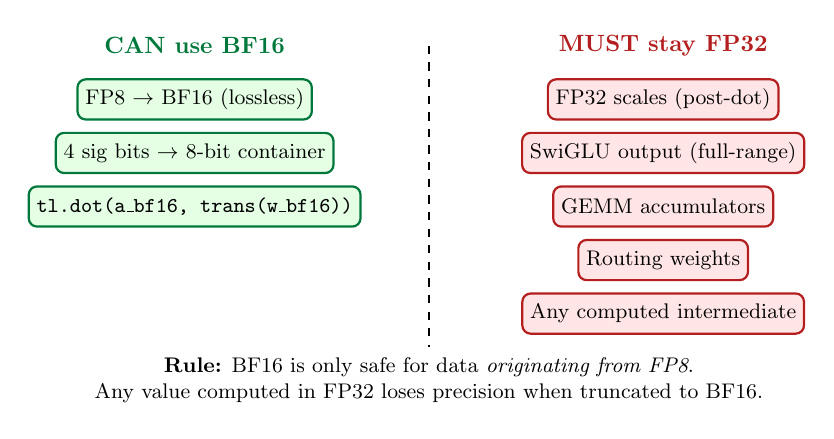
\begin{tikzpicture}[
    safe/.style={rectangle, draw=deepgreen, thick, fill=green!10, 
                 rounded corners=3pt, minimum height=0.6cm, font=\small},
    unsafe/.style={rectangle, draw=deepred, thick, fill=red!10, 
                   rounded corners=3pt, minimum height=0.6cm, font=\small},
    scale=0.85, transform shape
]

% Safe column
\node[font=\bfseries, deepgreen] at (-3.5, 2.5) {CAN use BF16};
\node[safe] at (-3.5, 1.7) {FP8 $\to$ BF16 (lossless)};
\node[safe] at (-3.5, 0.9) {4 sig bits $\to$ 8-bit container};
\node[safe] at (-3.5, 0.1) {\texttt{tl.dot(a\_bf16, trans(w\_bf16))}};

% Unsafe column
\node[font=\bfseries, deepred] at (3.5, 2.5) {MUST stay FP32};
\node[unsafe] at (3.5, 1.7) {FP32 scales (post-dot)};
\node[unsafe] at (3.5, 0.9) {SwiGLU output (full-range)};
\node[unsafe] at (3.5, 0.1) {GEMM accumulators};
\node[unsafe] at (3.5, -0.7) {Routing weights};
\node[unsafe] at (3.5, -1.5) {Any computed intermediate};

% Divider
\draw[thick, dashed] (0, 2.5) -- (0, -2);

% Bottom explanation
\node[font=\small, align=center] at (0, -2.5) {
    \textbf{Rule:} BF16 is only safe for data \emph{originating from FP8}.\\
    Any value computed in FP32 loses precision when truncated to BF16.
};

\end{tikzpicture}
\end{center}

\vspace{0.2cm}
\begin{alertblock}{Sub-11 Failure: BF16 SwiGLU Output}
SwiGLU output has full FP32 range. BF16 truncation $\to$ 0.13\% error per element 
$\times$ 2048 accumulation steps in GEMM2 $\to$ exceeds numerical tolerance.
\end{alertblock}
\end{frame}

% ═══════════════════════════════════════════════════════════════════════════ %
\section{Current Architecture (Sub-12)}
% ═══════════════════════════════════════════════════════════════════════════ %

\begin{frame}{Sub-12: Final Working Architecture}
\begin{center}
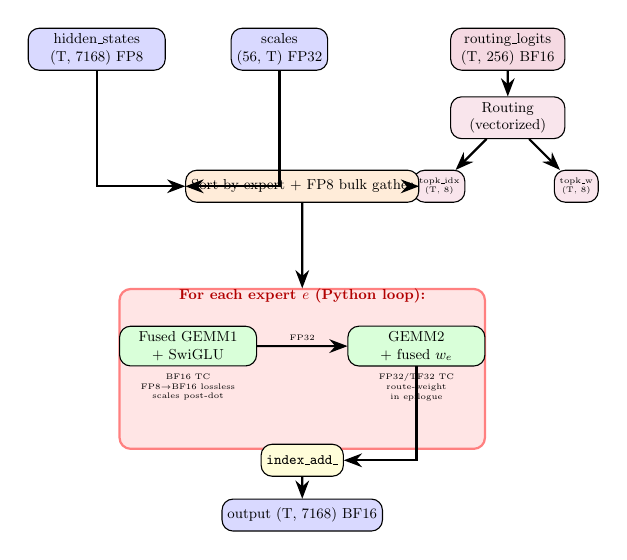
\begin{tikzpicture}[
    box/.style={rectangle, draw, rounded corners=4pt, font=\small, 
                align=center, minimum height=0.7cm},
    arrow/.style={->, thick, >=Stealth},
    scale=0.58, transform shape
]

% Input
\node[box, fill=blue!15, minimum width=3cm] (hs) at (0, 0) 
    {hidden\_states\\(T, 7168) FP8};
\node[box, fill=blue!15, minimum width=2cm] (sc) at (4, 0) 
    {scales\\(56, T) FP32};

% Routing branch
\node[box, fill=purple!15, minimum width=2.5cm] (rl) at (9, 0) 
    {routing\_logits\\(T, 256) BF16};
\node[box, fill=purple!10, minimum width=2.5cm] (rt) at (9, -1.5) 
    {Routing\\(vectorized)};
\draw[arrow] (rl) -- (rt);

% Routing output
\node[box, fill=purple!10, font=\tiny] (idx) at (7.5, -3) 
    {topk\_idx\\(T, 8)};
\node[box, fill=purple!10, font=\tiny] (wts) at (10.5, -3) 
    {topk\_w\\(T, 8)};
\draw[arrow] (rt) -- (idx);
\draw[arrow] (rt) -- (wts);

% Sort + Gather
\node[box, fill=orange!15, minimum width=4cm] (sort) at (4.5, -3) 
    {Sort by expert + FP8 bulk gather};
\draw[arrow] (hs) |- (sort);
\draw[arrow] (sc) |- (sort);
\draw[arrow] (idx) -- (sort);

% Expert loop
\node[box, fill=red!10, minimum width=8cm, minimum height=3.5cm, 
      draw=red!50, thick] (loop) at (4.5, -7) {};
\node[font=\small\bfseries, red!70!black] at (4.5, -5.4) 
    {For each expert $e$ (Python loop):};

% Fused GEMM1+SwiGLU
\node[box, fill=green!15, minimum width=3cm] (g1) at (2, -6.5) 
    {Fused GEMM1\\+ SwiGLU};
\node[font=\tiny, align=center] at (2, -7.4) 
    {BF16 TC\\FP8$\to$BF16 lossless\\scales post-dot};

% GEMM2 + fused weight
\node[box, fill=green!15, minimum width=3cm] (g2) at (7, -6.5) 
    {GEMM2\\+ fused $w_e$};
\node[font=\tiny, align=center] at (7, -7.4) 
    {FP32/TF32 TC\\route-weight\\in epilogue};

\draw[arrow] (sort) -- (loop.north);
\draw[arrow] (g1) -- node[above, font=\tiny] {FP32} (g2);

% Scatter
\node[box, fill=yellow!15] (scatter) at (4.5, -9) 
    {\texttt{index\_add\_}};
\draw[arrow] (g2) |- (scatter);

% Output
\node[box, fill=blue!15, minimum width=3cm] (out) at (4.5, -10.2) 
    {output (T, 7168) BF16};
\draw[arrow] (scatter) -- (out);

\end{tikzpicture}
\end{center}
\end{frame}

% ═══════════════════════════════════════════════════════════════════════════ %
\begin{frame}[t]{Bandwidth Audit: Where Every Byte Goes}
\begin{center}
\scriptsize
\begin{tabular}{llrl}
\toprule
\textbf{Operation} & \textbf{Size ($T_k{=}256$)} & \textbf{MB} & \textbf{Notes} \\
\midrule
\multicolumn{4}{l}{\textit{Gather (once per expert):}} \\
\quad FP8 tokens & $256 \times 7168 \times 1$ & 1.8 & 4$\times$ cheaper than FP32 \\
\quad Scales & $56 \times 256 \times 4$ & 0.06 & Tiny \\
\quad Route weights & $256 \times 4$ & 0.001 & Negligible \\
\midrule
\multicolumn{4}{l}{\textit{GEMM1+SwiGLU (56 K-iterations):}} \\
\quad A loads (FP8) & $56 \times 64 \times 128 \times 1$ & 7.2 & Shared gate/up \\
\quad W loads (FP8, $\times$2) & $56 \times 2 \times 128 \times 128 \times 1$ & 28.7 & 
    \textcolor{deepred}{Dominant} \\
\quad C output (FP32) & $256 \times 2048 \times 4$ & 2.1 & \\
\midrule
\multicolumn{4}{l}{\textit{GEMM2 (16 K-iterations):}} \\
\quad C loads (FP32) & $16 \times 64 \times 128 \times 4$ & 29.4 & 
    \textcolor{deepred}{Dominant} \\
\quad W loads (FP8) & $16 \times 128 \times 128 \times 1$ & 14.7 & \\
\quad O output (FP32) & $256 \times 7168 \times 4$ & 7.3 & 
    Includes fused $w_e$ \\
\midrule
\multicolumn{4}{l}{\textit{Post-GEMM2 (Sub-9 vs Sub-12):}} \\
\quad \sout{$o \times w_e$ multiply} & \sout{$256 \times 7168 \times 4 \times 2$} & 
    \sout{14.7} & \textcolor{deepgreen}{Eliminated in Sub-12} \\
\quad \texttt{index\_add\_} & $256 \times 7168 \times 4$ & 7.3 & \\
\midrule
\textbf{Total per expert} & & \textbf{$\sim$98} & (was $\sim$113 in Sub-9) \\
\bottomrule
\end{tabular}
\end{center}
\end{frame}

% ═══════════════════════════════════════════════════════════════════════════ %
\section{Lessons Learned}
% ═══════════════════════════════════════════════════════════════════════════ %

\begin{frame}[t]{Hard-Won Rules for Triton MoE Kernels (I)}
\small
\begin{columns}[T]
\column{0.48\textwidth}
\begin{block}{Precision Rules}
\begin{enumerate}
    \item FP8 $\to$ BF16 is lossless
    \item Never truncate FP32-computed values to BF16
    \item Factor scales out of dot products
    \item Keep accumulators FP32
    \item Convert only at final output
\end{enumerate}
\end{block}
\column{0.48\textwidth}
\begin{block}{Memory Rules}
\begin{enumerate}
    \item Use coalesced loads in stride-1 dimension
    \item Prefer \texttt{tl.trans()} over transposed loads
    \item Count SMEM budget before tuning stages
    \item Use FP8 gathers to reduce bandwidth
    \item Avoid allocations in expert loop
\end{enumerate}
\end{block}
\end{columns}
\end{frame}

\begin{frame}[t]{Hard-Won Rules for Triton MoE Kernels (II)}
\small
\begin{columns}[T]
\column{0.48\textwidth}
\begin{block}{Triton Pitfalls}
\begin{enumerate}
    \item \texttt{tl.dot} operands must match expected dtypes
    \item Some dtype+transpose paths can silently degrade results
    \item Dynamic loops can block compiler optimization
    \item \texttt{tl.atomic\_add} with scattered 2D patterns is fragile
\end{enumerate}
\end{block}
\column{0.48\textwidth}
\begin{block}{Architecture Rules}
\begin{enumerate}
    \item Match tile sizes to scale quantum (128)
    \item Tune \texttt{num\_stages} under SMEM limits
    \item Balance \texttt{num\_warps} with tile geometry
    \item Prefer robust scatter paths when possible
\end{enumerate}
\end{block}
\end{columns}
\end{frame}

\begin{frame}[t]{Implementation Guardrails (Validation)}
\small
\begin{columns}[T]
\column{0.48\textwidth}
\begin{block}{Numerical Validation Checklist}
\begin{itemize}
    \item Compare against FP32 reference output
    \item Track max/mean absolute error after each fusion
    \item Verify routing normalization before dispatch
    \item Stress-test skewed expert token distributions
\end{itemize}
\end{block}
\column{0.48\textwidth}
\begin{block}{Performance Validation Checklist}
\begin{itemize}
    \item Separate launch overhead from kernel runtime
    \item Measure achieved bandwidth vs roofline
    \item Profile L2 hit-rate with tile-order changes
    \item Re-audit stage-level read/write bytes
\end{itemize}
\end{block}
\end{columns}
\end{frame}

\begin{frame}[t]{Implementation Guardrails (Regression Traps)}
\small
\begin{alertblock}{Common Regression Traps}
\begin{itemize}
    \item Hidden dtype casts in helper kernels
    \item Non-coalesced accesses after pointer rewrites
    \item Temporary tensors accidentally reintroduced
    \item Over-aggressive stage/warp settings
\end{itemize}
\end{alertblock}

\begin{exampleblock}{Practical Rule}
Treat every optimization as a three-way check:
\textbf{correctness} + \textbf{memory traffic} + \textbf{occupancy}.
\end{exampleblock}
\end{frame}

% ═══════════════════════════════════════════════════════════════════════════ %
\section{Future Directions: Grouped GEMM}
% ═══════════════════════════════════════════════════════════════════════════ %

\begin{frame}[fragile,t]{The Remaining Bottleneck: Python Expert Loop (Current Path)}
\small
\begin{alertblock}{Current pattern: up to 32 experts in Python loop}
\begin{lstlisting}[basicstyle=\ttfamily\scriptsize]
for i in range(unique_experts.numel()):
    _launch_fused_gemm1_swiglu(...)
    _launch_gemm2_weighted(...)
    accum.index_add_(...)
\end{lstlisting}
\end{alertblock}

\begin{itemize}
    \item Kernel launch overhead accumulates quickly
    \item Small-$T_k$ experts can become launch-bound
    \item SMs idle between dispatches
\end{itemize}
\end{frame}

\begin{frame}[t]{The Remaining Bottleneck: Python Expert Loop (Direction)}
\small
\begin{exampleblock}{Direction: Grouped/Persistent GEMM}
Replace per-expert host loop with one scheduler-driven kernel per operation,
so all experts are processed via a shared tile worklist.
\end{exampleblock}

\begin{itemize}
    \item Reduces launch count substantially
    \item Improves overlap and occupancy
    \item Better fit for irregular MoE workloads
\end{itemize}
\end{frame}

% ═══════════════════════════════════════════════════════════════════════════ %
\begin{frame}[t]{Grouped GEMM: How It Works (Scheduler View)}
\begin{center}
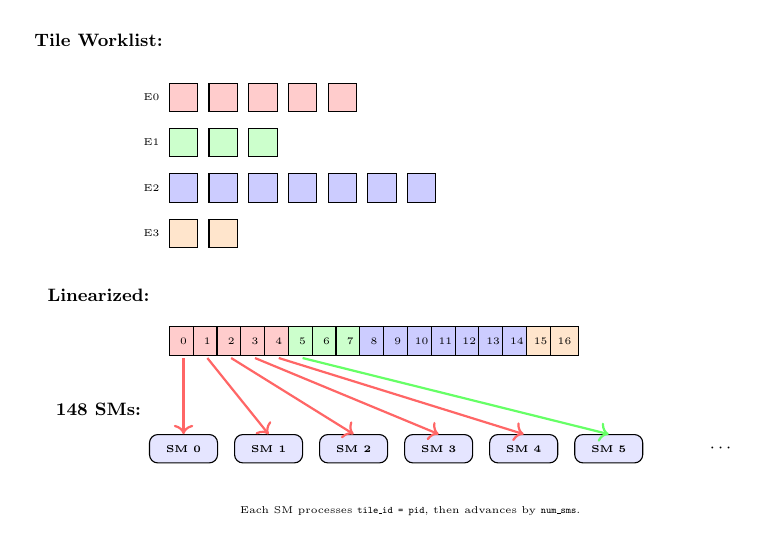
\begin{tikzpicture}[scale=0.72, transform shape,
    tile/.style={rectangle, draw, minimum width=0.5cm, minimum height=0.5cm,
                 font=\tiny},
    sm/.style={rectangle, draw, rounded corners=3pt, minimum width=1.2cm,
               minimum height=0.5cm, font=\tiny\bfseries, fill=blue!10}]

\node[font=\small\bfseries] at (-1.5, 3) {Tile Worklist:};
\foreach \i in {0,...,4} {\node[tile, fill=red!20] at (\i*0.7, 2) {};}
\node[font=\tiny, left] at (-0.3, 2) {E0};
\foreach \i in {0,...,2} {\node[tile, fill=green!20] at (\i*0.7, 1.2) {};}
\node[font=\tiny, left] at (-0.3, 1.2) {E1};
\foreach \i in {0,...,6} {\node[tile, fill=blue!20] at (\i*0.7, 0.4) {};}
\node[font=\tiny, left] at (-0.3, 0.4) {E2};
\foreach \i in {0,...,1} {\node[tile, fill=orange!20] at (\i*0.7, -0.4) {};}
\node[font=\tiny, left] at (-0.3, -0.4) {E3};

\node[font=\small\bfseries] at (-1.5, -1.5) {Linearized:};
\foreach \i/\c in {0/red!20, 1/red!20, 2/red!20, 3/red!20, 4/red!20,
                   5/green!20, 6/green!20, 7/green!20,
                   8/blue!20, 9/blue!20, 10/blue!20, 11/blue!20,
                   12/blue!20, 13/blue!20, 14/blue!20,
                   15/orange!20, 16/orange!20} {
    \node[tile, fill=\c] at (\i*0.42, -2.3) {\i};
}

\node[font=\small\bfseries] at (-1.5, -3.5) {148 SMs:};
\foreach \i in {0,...,5} {\node[sm] (sm\i) at (\i*1.5, -4.2) {SM \i};}
\node[font=\small] at (9.5, -4.2) {$\cdots$};
\draw[->, thick, red!60] (0*0.42, -2.6) -- (sm0.north);
\draw[->, thick, red!60] (1*0.42, -2.6) -- (sm1.north);
\draw[->, thick, red!60] (2*0.42, -2.6) -- (sm2.north);
\draw[->, thick, red!60] (3*0.42, -2.6) -- (sm3.north);
\draw[->, thick, red!60] (4*0.42, -2.6) -- (sm4.north);
\draw[->, thick, green!60] (5*0.42, -2.6) -- (sm5.north);

\node[font=\tiny, align=center] at (4, -5.3)
    {Each SM processes \texttt{tile\_id = pid}, then advances by \texttt{num\_sms}.};
\end{tikzpicture}
\end{center}
\end{frame}

\begin{frame}[t]{Grouped GEMM: How It Works (Trade-offs)}
\begin{columns}[T]
\column{0.48\textwidth}
\begin{block}{Benefits}
\begin{itemize}
    \item 64 launches $\to$ 2 launches
    \item Higher SM occupancy with less idle time
    \item Better L2 behavior from structured tile traversal
    \item Scales naturally with active experts
\end{itemize}
\end{block}

\column{0.48\textwidth}
\begin{alertblock}{Challenges}
\begin{itemize}
    \item Loop bounds and indexing logic must stay compiler-friendly
    \item Requires precomputed cumulative offsets
    \item Tile-to-expert mapping adds register pressure
    \item Debugging scheduler logic is more complex
\end{itemize}
\end{alertblock}
\end{columns}
\end{frame}

% ═══════════════════════════════════════════════════════════════════════════ %
\begin{frame}[fragile,t]{Grouped GEMM: Tile-to-Expert Mapping (Host Setup)}
\small
\begin{block}{Precomputed on Host (Python)}
\begin{lstlisting}[basicstyle=\ttfamily\scriptsize]
# For each expert, compute number of M-tiles and N-tiles
# expert_offsets: cumulative sum of token counts
# tile_offsets[e] = cumsum of (m_tiles_e * n_tiles) for experts 0..e-1
# Total tiles = sum over all experts of (m_tiles_e * n_tiles)
total_tiles = sum(cdiv(Tk_e, BLOCK_M) * cdiv(N, BLOCK_N) for each expert)
\end{lstlisting}
\end{block}

\begin{itemize}
    \item Host precomputation turns irregular per-expert work into a compact tile worklist.
    \item Kernel can fetch work by tile id instead of launching one grid per expert.
\end{itemize}
\end{frame}

\begin{frame}[fragile,t]{Grouped GEMM: Tile-to-Expert Mapping (Kernel Loop)}
\small
\begin{block}{Inside Kernel (Triton)}
\begin{lstlisting}[basicstyle=\ttfamily\scriptsize]
pid = tl.program_id(0)
tile_id = pid
while tile_id < total_tiles:
    expert_idx = find_expert(tile_id, tile_offsets_ptr, num_experts)
    local_tile = tile_id - tile_offsets[expert_idx]
    m_block = local_tile // n_tiles
    n_block = local_tile % n_tiles
    compute_tile(expert_idx, m_block, n_block, ...)
    tile_id += NUM_SMS  # persistent: advance by grid size
\end{lstlisting}
\end{block}

\textbf{Key constraint:} use compiler-safe control flow for expert lookup
(\texttt{tl.constexpr} bounds or table-driven \texttt{while} design).
\end{frame}

% ═══════════════════════════════════════════════════════════════════════════ %
\begin{frame}[fragile,t]{Other Future Optimizations (I)}
\small
\begin{columns}[T]
\column{0.49\textwidth}
\begin{block}{\texttt{tl.dot\_scaled} (B200 Native)}
\begin{lstlisting}[basicstyle=\ttfamily\scriptsize]
acc = tl.dot_scaled(
    a_fp8, scale_a,
    w_fp8, scale_w,
)
\end{lstlisting}
Requires MXFP8 (E8M0) scale format; not directly compatible with arbitrary FP32 scale layouts.
\end{block}

\column{0.49\textwidth}
\begin{block}{CUDA Streams Overlap}
\begin{lstlisting}[basicstyle=\ttfamily\scriptsize]
with stream_a:
    gemm1_swiglu(expert_e+1)
with stream_b:
    gemm2_weighted(expert_e)
\end{lstlisting}
Overlaps adjacent-stage expert work to hide latency.
\end{block}
\end{columns}
\end{frame}

\begin{frame}[t]{Other Future Optimizations (II)}
\small
\begin{columns}[T]
\column{0.49\textwidth}
\begin{block}{DeepGEMM Integration}
\begin{itemize}
    \item Grouped GEMM in a single launch path
    \item FP8 block-scale support
    \item JIT specialization to exact problem shapes
\end{itemize}
\end{block}

\begin{block}{MXFP4 Weights}
\begin{itemize}
    \item 2$\times$ less weight bandwidth vs FP8
    \item B200 hardware acceleration path
    \item Requires retraining/calibration support
\end{itemize}
\end{block}

\column{0.49\textwidth}
\begin{block}{L2 Cache-Aware Tiling}
\begin{itemize}
    \item 1D swizzled launch ordering (\texttt{GROUP\_SIZE\_M})
    \item Improves weight tile reuse in L2
    \item Typical 15--30\% L2 hit-rate gain
\end{itemize}
\end{block}
\end{columns}
\end{frame}

% ═══════════════════════════════════════════════════════════════════════════ %
\section{Summary}
% ═══════════════════════════════════════════════════════════════════════════ %

\begin{frame}[t]{Optimization Summary: What We Achieved (Table)}
\footnotesize
\begin{center}
\begin{tabular}{lccl}
\toprule
\textbf{Optimization} & \textbf{Sub} & \textbf{BW Saved/Expert} & \textbf{Status} \\
\midrule
Fused GEMM1 + SwiGLU & 9 & 8.4 MB & \textcolor{deepgreen}{\checkmark\ Working} \\
BF16 TC (factored scales) & 9 & $\sim$2$\times$ TFLOPS & \textcolor{deepgreen}{\checkmark\ Working} \\
FP8 bulk gather & 9 & 5.4 MB & \textcolor{deepgreen}{\checkmark\ Working} \\
Route-weight fusion & 12 & 14.7 MB & \textcolor{deepgreen}{\checkmark\ Working} \\
\midrule
Transposed loads & 10 & --- & \textcolor{deepred}{$\times$ BW blowup} \\
BF16 SwiGLU output & 11 & 14.7 MB & \textcolor{deepred}{$\times$ Precision loss} \\
\texttt{tl.atomic\_add} scatter & 10 & 7.3 MB & \textcolor{deepred}{$\times$ Runtime crash} \\
\texttt{num\_stages=4} & 12 & --- & \textcolor{deepred}{$\times$ SMEM overflow} \\
\bottomrule
\end{tabular}
\end{center}
\end{frame}

\begin{frame}[t]{Optimization Summary: What We Achieved (Net Gain)}
\small
\begin{exampleblock}{Total Bandwidth Reduction: Sub-7 $\to$ Sub-12}
$\sim$113 MB/expert $\to$ $\sim$98 MB/expert ($\approx$13\% reduction per expert).
At 20 active experts: $\sim$2.26 GB $\to$ $\sim$1.96 GB, saving about 300 MB per forward pass.
\end{exampleblock}

\begin{block}{Compute Impact}
BF16 tensor-core path delivers roughly 2$\times$ GEMM1 throughput while preserving target numerical behavior.
\end{block}
\end{frame}

% ═══════════════════════════════════════════════════════════════════════════ %
\begin{frame}[t]{The Complete Precision Chain}

\begin{center}
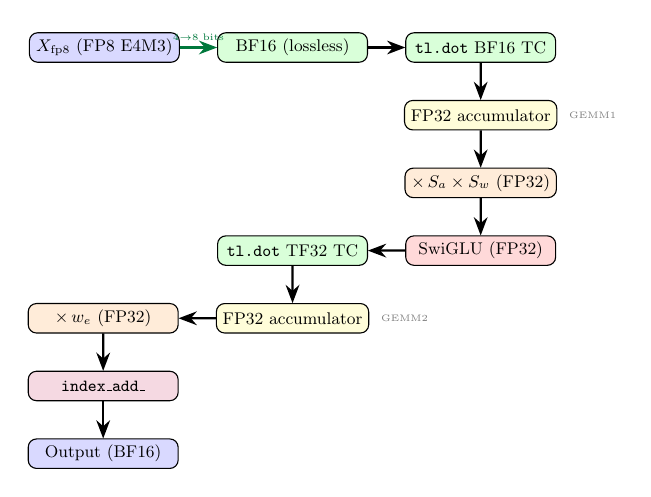
\begin{tikzpicture}[
    node distance=0.7cm,
    box/.style={rectangle, draw, rounded corners=3pt, font=\small, 
                align=center, minimum width=2.8cm, minimum height=0.55cm},
    arrow/.style={->, thick, >=Stealth},
    scale=0.68, transform shape
]

\node[box, fill=blue!15] (fp8a) {$X_{\text{fp8}}$ (FP8 E4M3)};
\node[box, fill=green!15, right=of fp8a] (bf16a) {BF16 (lossless)};
\node[box, fill=green!15, right=of bf16a] (dot1) {\texttt{tl.dot} BF16 TC};
\node[box, fill=yellow!15, below=of dot1] (acc1) {FP32 accumulator};
\node[box, fill=orange!15, below=of acc1] (scale) {$\times\, S_a \times S_w$ (FP32)};
\node[box, fill=red!15, below=of scale] (swiglu) {SwiGLU (FP32)};
\node[box, fill=green!15, left=of swiglu] (dot2) {\texttt{tl.dot} TF32 TC};
\node[box, fill=yellow!15, below=of dot2] (acc2) {FP32 accumulator};
\node[box, fill=orange!15, left=of acc2] (routew) {$\times\, w_e$ (FP32)};
\node[box, fill=purple!15, below=of routew] (scatter) {\texttt{index\_add\_}};
\node[box, fill=blue!15, below=of scatter] (output) {Output (BF16)};

\draw[arrow, deepgreen] (fp8a) -- node[above, font=\tiny] {4$\to$8 bits} (bf16a);
\draw[arrow] (bf16a) -- (dot1);
\draw[arrow] (dot1) -- (acc1);
\draw[arrow] (acc1) -- (scale);
\draw[arrow] (scale) -- (swiglu);
\draw[arrow] (swiglu) -- (dot2);
\draw[arrow] (dot2) -- (acc2);
\draw[arrow] (acc2) -- (routew);
\draw[arrow] (routew) -- (scatter);
\draw[arrow] (scatter) -- (output);

% Type annotations
\node[font=\tiny, gray, right=0.1cm of acc1] {GEMM1};
\node[font=\tiny, gray, right=0.1cm of acc2] {GEMM2};

\end{tikzpicture}
\end{center}

\vspace{0.2cm}
\centering\small
\textbf{Every arrow is precision-safe.} The only truncation is the final BF16 cast.
\end{frame}

% ═══════════════════════════════════════════════════════════════════════════ %
\begin{frame}{Key Takeaway}

\begin{center}
\Large

\vspace{1cm}

\textbf{GPU kernel optimization is a constrained search:}

\vspace{0.5cm}

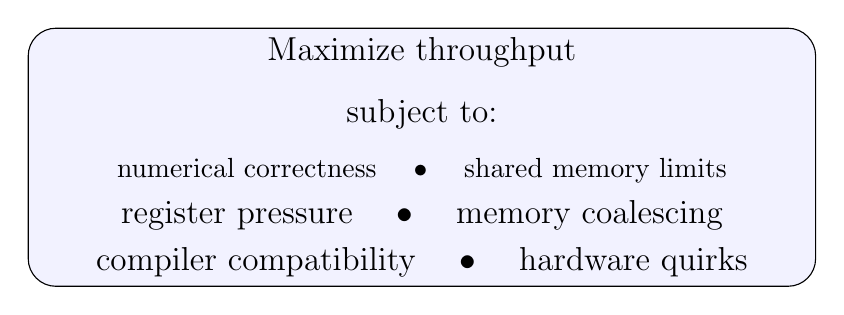
\begin{tikzpicture}
\node[draw, rounded corners=10pt, fill=blue!5, minimum width=10cm, 
      minimum height=3cm, font=\large, align=center] {
    Maximize throughput\\[0.3cm]
    subject to:\\[0.2cm]
    \normalsize
    numerical correctness $\quad\bullet\quad$ 
    shared memory limits\\[0.1cm]
    register pressure $\quad\bullet\quad$ 
    memory coalescing\\[0.1cm]
    compiler compatibility $\quad\bullet\quad$ 
    hardware quirks
};
\end{tikzpicture}

\vspace{0.5cm}

\normalsize
\textit{Every ``obvious'' optimization must be validated against\\
all constraints simultaneously.}

\end{center}
\end{frame}

% ═══════════════════════════════════════════════════════════════════════════ %
\begin{frame}{}
\begin{center}
\Huge\bfseries Thank You

\vspace{1cm}
\large
Questions?

\vspace{1cm}
\normalsize
\texttt{Humming Bird Team --- Presented by Vansh Nawander}
\end{center}
\end{frame}

\end{document}